\documentclass[answers,12pt]{exam}

\setlength{\parindent}{0cm} % global indent value

\usepackage{graphicx}
\usepackage{mhchem}
\usepackage{wrapfig}

\pagestyle{headandfoot}
\runningheadrule
\firstpageheader{name:\fillin[][4cm]}{period:\fillin[][1cm]}{Unit 2: Combustion}
\runningheader{Unit 2: Combustion}
{Class Notes}
{Page \thepage\ of \numpages}
\firstpagefooter{}{}{}
\runningfooter{PACS}{Mr. Maxwell}{page \thepage\ of \numpages}


\begin{document}

\section*{Lesson 2.1 Computing the Energy in Food}

\begin{itemize}
    \item The modern metric unit of energy is the \fillin[joule]. 
    \item An older unit of energy is the \fillin[calorie].
    \item To convert use: \fillin[1] calorie = \fillin[4.2] joules
    \item A food calorie = 1000 energy calories = 1 kilocalorie = 1 kcal
\end{itemize}
    

\begin{wrapfigure}{r}{0.5\textwidth} %this figure will be at the right
    \centering
    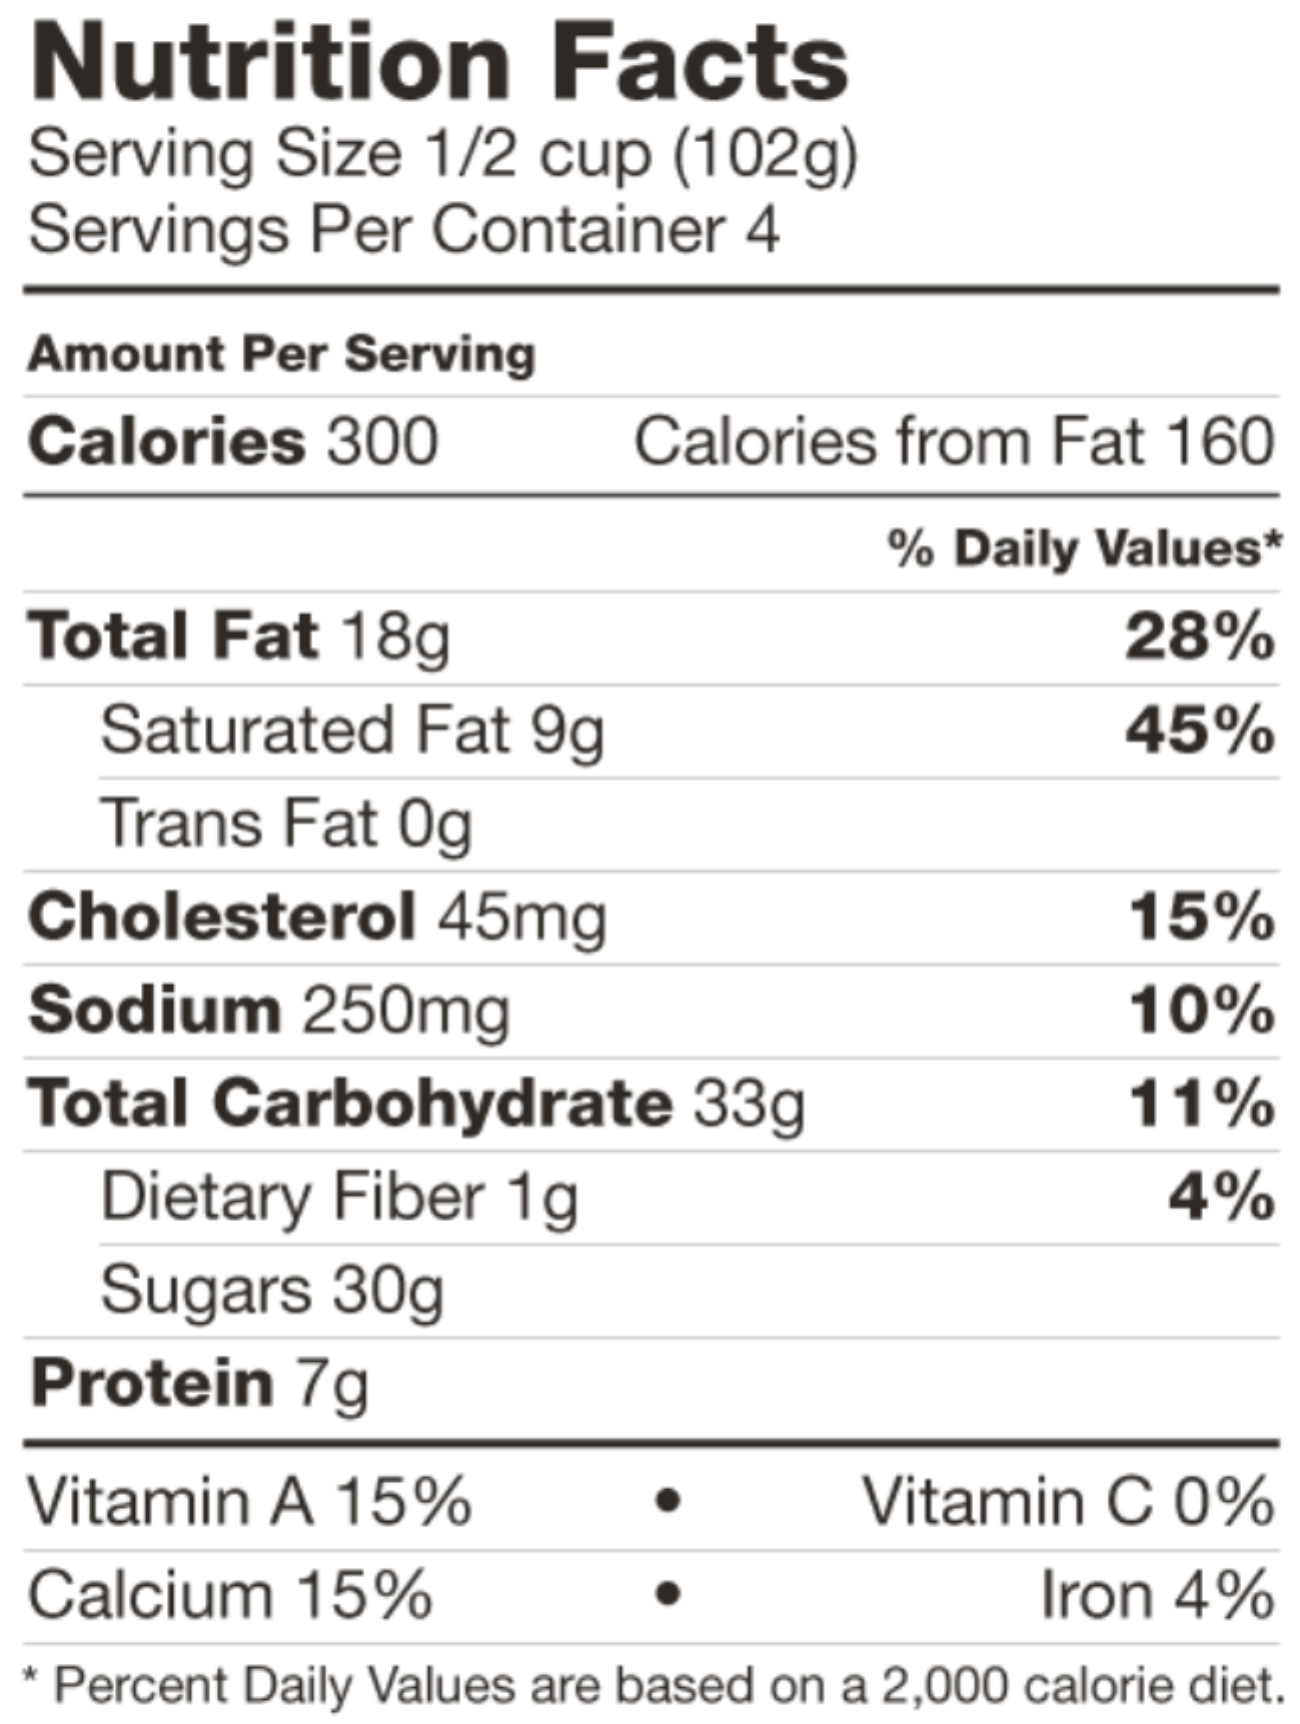
\includegraphics[width=0.35\textwidth]{food_label.png}
\end{wrapfigure}


Find the \textbf{grams per serving} \\ 

Find the food \textbf{calories per serving} on the label - remember that these are actually kcal of energy. \\

Compute the kcal per gram:

$$ calories \; per \; serving = \fillin[300] kcal $$
$$ grams \; per \; serving = \fillin[102] g $$

$$ \frac{calories \; per \; serving}{grams \; per \; serving} = \fillin[2.9] kcal/g  $$

\vspace{1cm}

\newpage

\section*{Lab Bingo}

\newpage

\section*{Lesson 2.2 Bio-fuel Lab}
\section*{Lesson 2.3 Combustion Conference}
\section*{Lesson 2.4 Combustion Video}

\begin{enumerate}
    \item  \fillin[] is a fuel used a lot in the past, and even today.
    \item  The three most widely used fuels today are \fillin[], \fillin[], and \fillin[].
    \item  A newer fuel often used in rockets is \fillin[].
    \item  When a fuel is burned it always combines with \fillin[].
    \item  Other products released during combustion are \fillin[] and \fillin[] that are emitted as a \fillin[].
    \item  A very fast combustion reaction is called an \fillin[].
    \item  We use fast reactions in \fillin[].
    \item  Combustion reactions are used for:  \fillin[], \fillin[], \fillin[], \fillin[], \fillin[], and \fillin[].
\end{enumerate}

\subsubsection*{Word Bank}

\begin{tabular}{ |c c c|}
    \hline
    car engines     & carbon dioxide    & coal\\ 
    cooking         & explosion         & gas\\ 
    heating         & heating water     & hydrogen\\ 
    manufacturing   & motor vehicles    & natural gas\\ 
    oil             & oxygen            & produce electricity\\ 
    water           & wood              & \\ 
    \hline    
\end{tabular}




















    
    
\end{document}